\subsection{Experimental Setup}
\label{sec:setup}

\subsubsection{System used}

We employ a server equipped with two Intel Xeon Gold 6226R processors, each featuring $16$ cores running at a clock speed of $2.90$ GHz. Each core is equipped with a $1$ MB L1 cache, a $16$ MB L2 cache, and a $22$ MB shared L3 cache. The system is configured with $376$ GB RAM and set up with CentOS Stream 8.


\subsubsection{Configuration}

We use 32-bit integers for vertex ids and 32-bit float for edge weights but use 64-bit floats for computations and hashtable values. We utilize $64$ threads to match the number of cores available on the system (unless specified otherwise). For compilation, we use GCC 8.5 and OpenMP 4.5.


\subsubsection{Dataset}

The graphs used in our experiments are given in Table \ref{tab:dataset}. These are sourced from the SuiteSparse Matrix Collection \cite{suite19}. In the graphs, number of vertices vary from $3.07$ to $214$ million, and number of edges vary from $25.4$ million to $3.80$ billion. We ensure edges to be undirected and weighted with a default of $1$.

\begin{table}[hbtp]
  \centering
  \caption{List of $13$ graphs obtained SuiteSparse Matrix Collection \cite{suite19} (directed graphs are marked with $*$). Here, $|V|$ is the number of vertices, $|E|$ is the number of edges (after adding reverse edges), $D_{avg}$ is the average degree, and $|\Gamma|$ is the number of communities obtained using Louvain algorithm.\ignore{In the table, B refers to a billion, M refers to a million and K refers a thousand.}}
  \label{tab:dataset}
  \begin{tabular}{|c||c|c|c|c|}
    \toprule
    \textbf{Graph} &
    \textbf{\textbf{$|V|$}} &
    \textbf{\textbf{$|E|$}} &
    \textbf{\textbf{$D_{avg}$}} &
    \textbf{\textbf{$|\Gamma|$}} \\
    % \textbf{$1 - \Gamma_G$} \\
    \midrule
    \multicolumn{5}{|c|}{\textbf{Web Graphs (LAW)}} \\ \hline
    indochina-2004$^*$ & 7.41M & 341M & 41.0 & 4.24K \\ \hline  % & \num{4.7e-4} & 2.9 GB
    uk-2002$^*$ & 18.5M & 567M & 16.1 & 42.8K \\ \hline  % & \num{9.6e-5} & 16 GB
    arabic-2005$^*$ & 22.7M & 1.21B & 28.2 & 3.66K \\ \hline  % & \num{5.5e-4} & 11 GB
    uk-2005$^*$ & 39.5M & 1.73B & 23.7 & 20.8K \\ \hline  % & \num{9.6e-5} & 16 GB
    webbase-2001$^*$ & 118M & 1.89B & 8.6 & 2.76M \\ \hline  % & \num{7.3e-7} & 18 GB
    it-2004$^*$ & 41.3M & 2.19B & 27.9 & 5.28K \\ \hline  % & \num{3.8e-4} & 19 GB
    sk-2005$^*$ & 50.6M & 3.80B & 38.5 & 3.47K \\ \hline  % & \num{5.8e-4} & 33 GB
    \multicolumn{5}{|c|}{\textbf{Social Networks (SNAP)}} \\ \hline
    com-LiveJournal & 4.00M & 69.4M & 17.4 & 2.54K \\ \hline  % & \num{7.9e-4} & 480 MB
    com-Orkut & 3.07M & 234M & 76.2 & 29 \\ \hline  % & \num{6.7e-2} & 1.7 GB
    \multicolumn{5}{|c|}{\textbf{Road Networks (DIMACS10)}} \\ \hline
    asia\_osm & 12.0M & 25.4M & 2.1 & 2.38K \\ \hline  % & \num{8.4e-4} & 200 MB
    europe\_osm & 50.9M & 108M & 2.1 & 3.05K \\ \hline  % & \num{6.6e-4} & 910 MB
    \multicolumn{5}{|c|}{\textbf{Protein k-mer Graphs (GenBank)}} \\ \hline
    kmer\_A2a & 171M & 361M & 2.1 & 21.2K \\ \hline  % & \num{9.4e-5} & 3.2 GB
    kmer\_V1r & 214M & 465M & 2.2 & 6.17K \\ \hline  % & \num{3.2e-4} & 4.2 GB
  \bottomrule
  \end{tabular}
\end{table}
% We convert directed graphs (marked with $*$) to undirected by duplicating edges in the reverse direction, and set the weight of each edge to $1$. and $F_{size}$ is size of the \textit{MatrixMarket} file

\begin{figure*}[hbtp]
  \centering
  \subfigure[Runtime in seconds (logarithmic scale) with \textit{Original Leiden}, \textit{igraph Leiden}, \textit{NetworKit Leiden}, and \textit{GVE-Leiden}]{
    \label{fig:leiden-compare--runtime}
    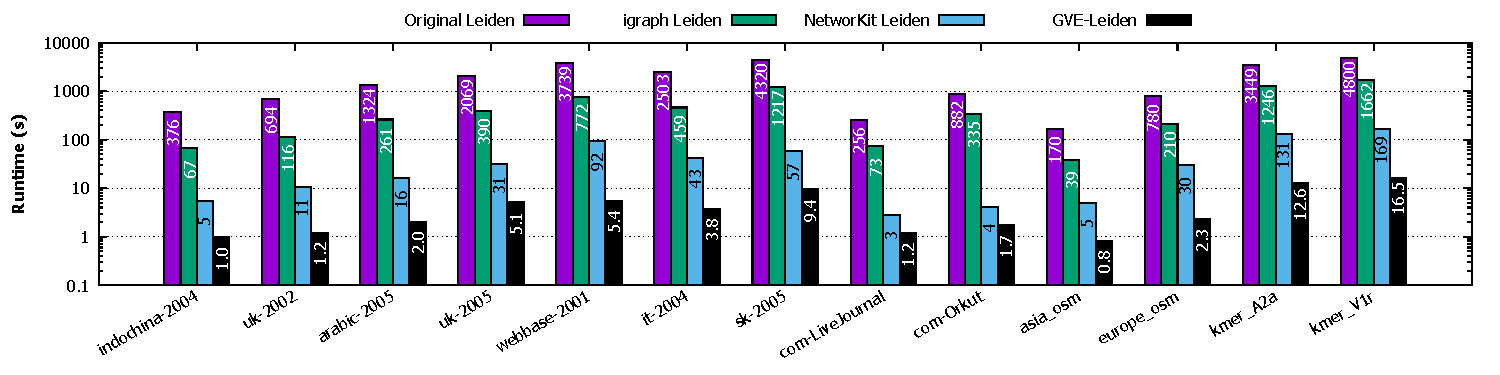
\includegraphics[width=0.98\linewidth]{out/leiden-runtime.pdf}
  } \\[-0ex]
  \subfigure[Speedup of \textit{GVE-Leiden} (logarithmic scale) with respect to \textit{Original Leiden}, \textit{igraph Leiden}, \textit{NetworKit Leiden}.]{
    \label{fig:leiden-compare--speedup}
    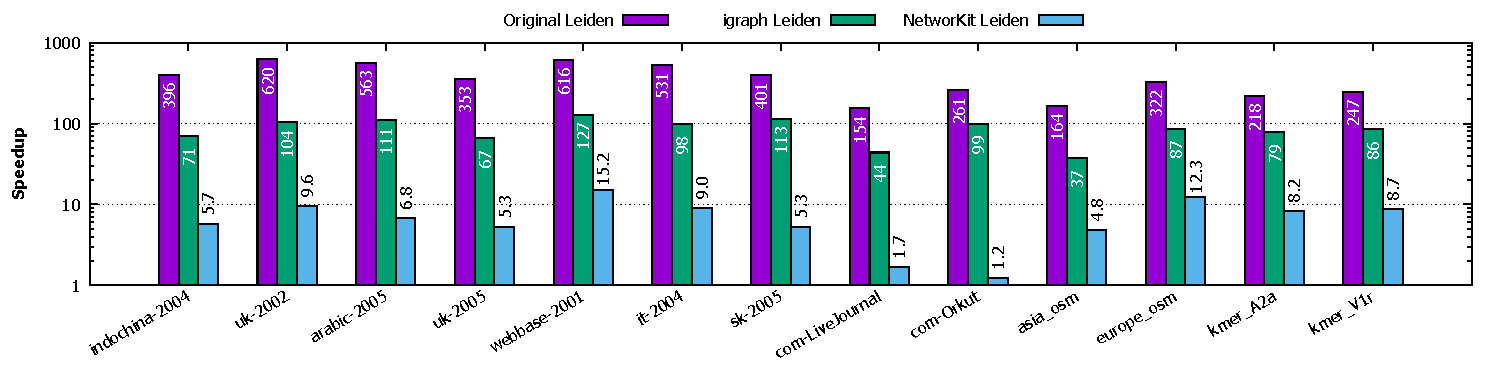
\includegraphics[width=0.98\linewidth]{out/leiden-speedup.pdf}
  } \\[-0ex]
  \subfigure[Modularity of communities obtained with \textit{Original Leiden}, \textit{igraph Leiden}, \textit{NetworKit Leiden}, and \textit{GVE-Leiden}.]{
    \label{fig:leiden-compare--modularity}
    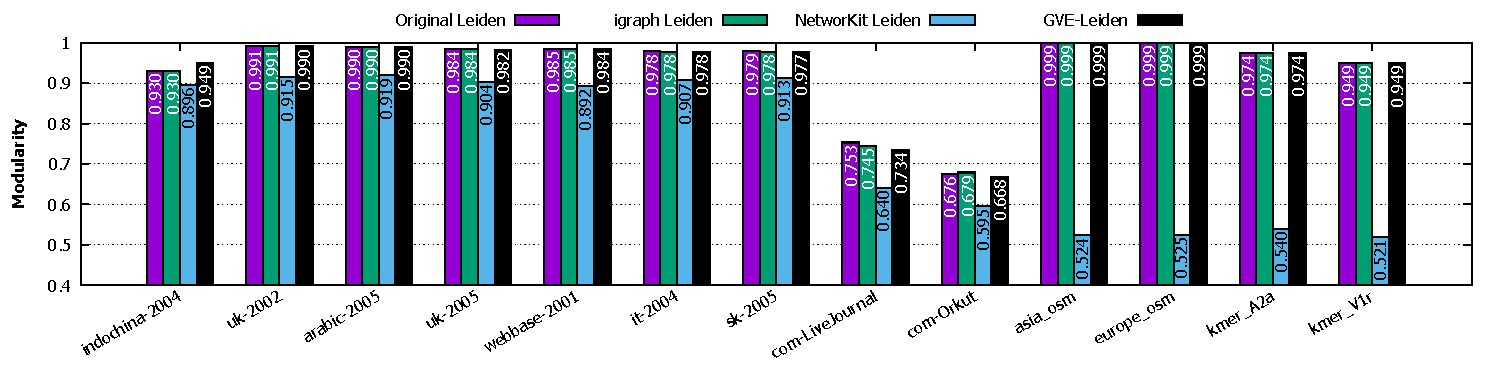
\includegraphics[width=0.98\linewidth]{out/leiden-modularity.pdf}
  } \\[-0ex]
  \subfigure[Fraction of disconnected communities (logarithmic scale) with \textit{Original Leiden}, \textit{igraph Leiden}, \textit{NetworKit Leiden}, and \textit{GVE-Leiden}.]{
    \label{fig:leiden-compare--disconnected}
    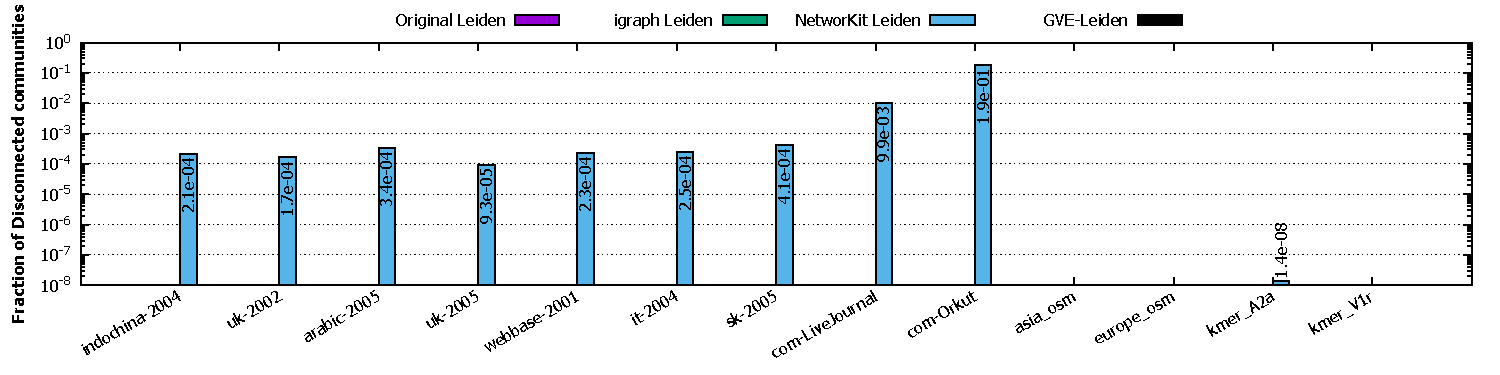
\includegraphics[width=0.98\linewidth]{out/leiden-disconnected.pdf}
  } \\[-2ex]
  \caption{Runtime in seconds (log-scale), speedup (log-scale), modularity, and fraction of disconnected communities (log-scale) with \textit{Original Leiden}, \textit{igraph Leiden}, \textit{NetworKit Leiden}, and \textit{GVE-Leiden} for each graph in the dataset.}
  \label{fig:leiden-compare}
\end{figure*}

\begin{figure*}[hbtp]
  \centering
  \subfigure[Runtime in seconds (logarithmic scale) with \textit{GVE-Louvain} and \textit{GVE-Leiden}]{
    \label{fig:gve-compare--runtime}
    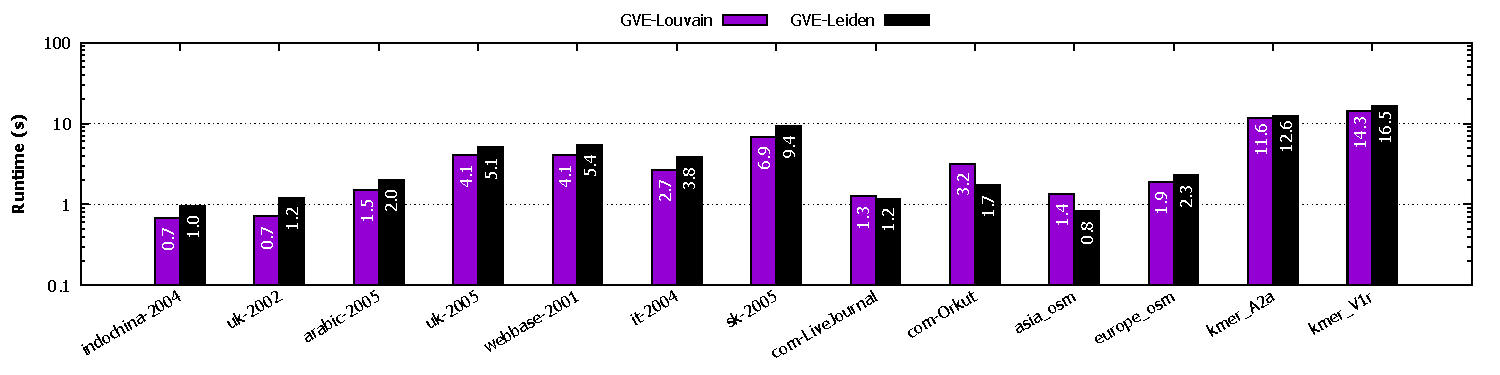
\includegraphics[width=0.98\linewidth]{out/gve-runtime.pdf}
  } \\[-0ex]
  \subfigure[Speedup of \textit{GVE-Leiden} with respect to \textit{GVE-Louvain}. \textit{GVE-Leiden} is generally slower (speedup < $1$) because of additional refinement phase.]{
    \label{fig:gve-compare--speedup}
    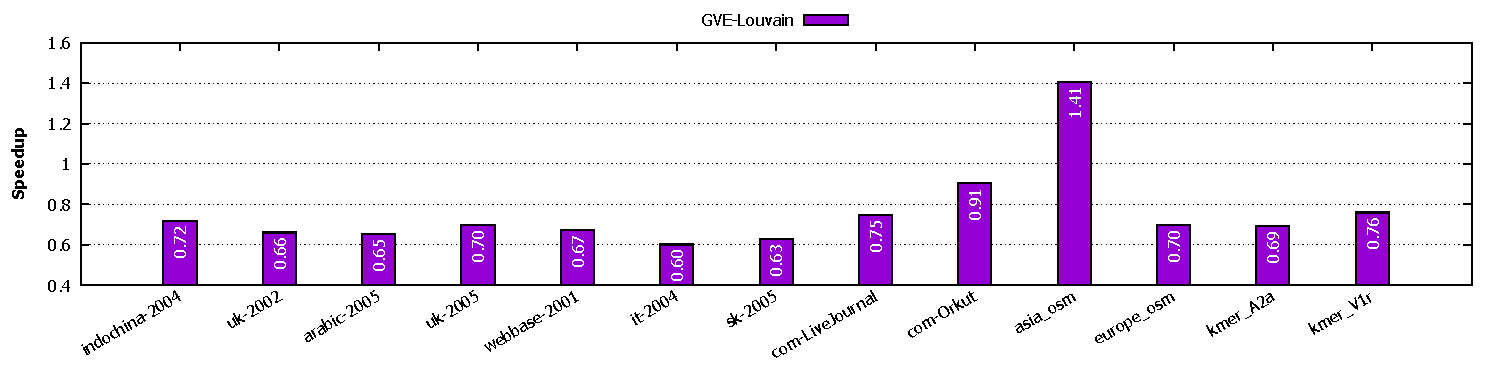
\includegraphics[width=0.98\linewidth]{out/gve-speedup.pdf}
  } \\[-0ex]
  \subfigure[Modularity of communities obtained with \textit{GVE-Louvain} and \textit{GVE-Leiden}.]{
    \label{fig:gve-compare--modularity}
    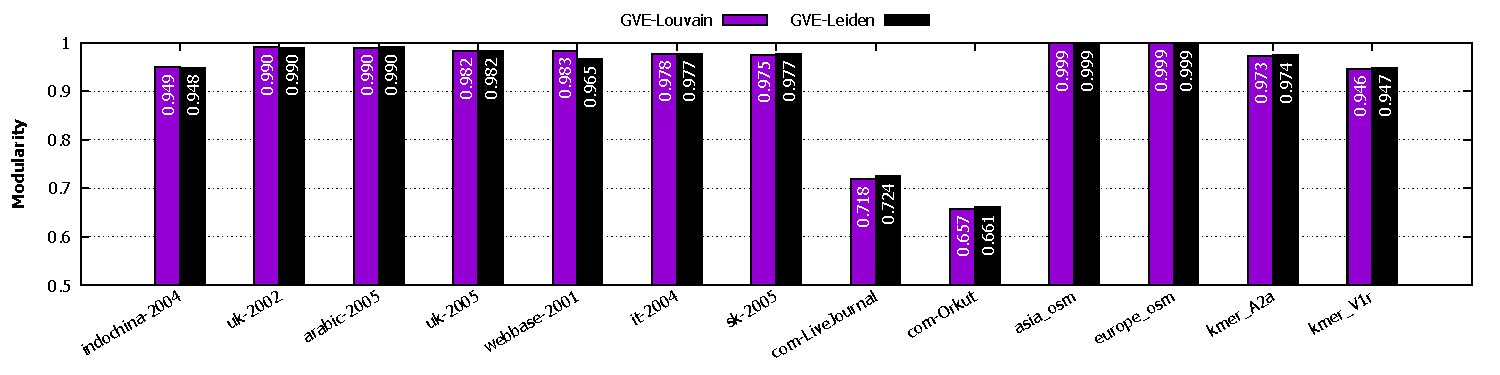
\includegraphics[width=0.98\linewidth]{out/gve-modularity.pdf}
  } \\[-0ex]
  \subfigure[Fraction of disconnected communities (logarithmic scale) with \textit{GVE-Louvain} and \textit{GVE-Leiden}.]{
    \label{fig:gve-compare--disconnected}
    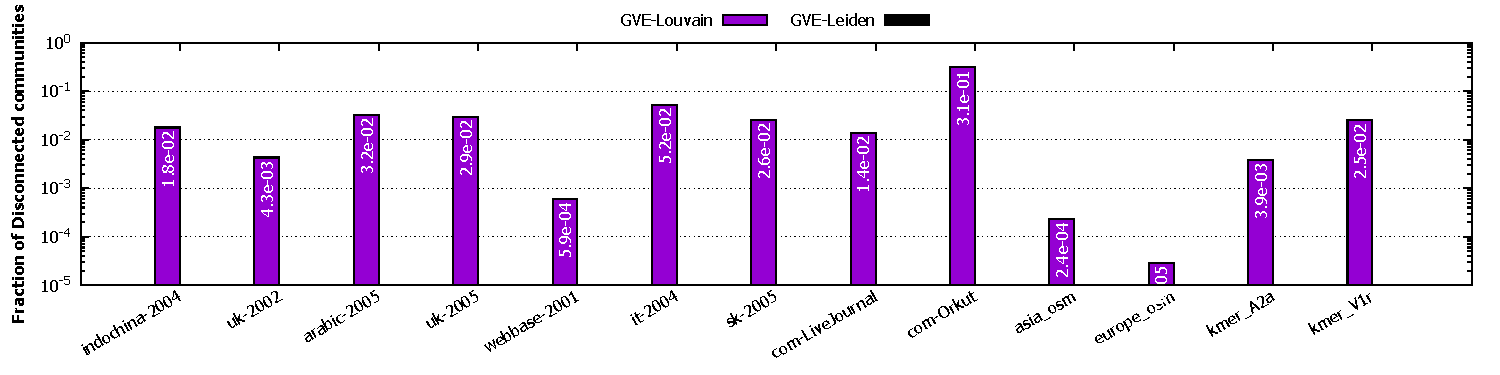
\includegraphics[width=0.98\linewidth]{out/gve-disconnected.pdf}
  } \\[-2ex]
  \caption{Runtime in seconds (log-scale), speedup, modularity, and fraction of disconnected communities (log-scale) with \textit{GVE-Louvain} and \textit{GVE-Leiden} for each graph in the dataset.}
  \label{fig:gve-compare}
\end{figure*}





\subsection{Comparing Performance of GVE-Leiden}

We now compare the performance of GVE-Leiden with the original Leiden \cite{com-traag19}, igraph Leiden \cite{csardi2006igraph}, and NetworKit Leiden \cite{staudt2016networkit}. For the original Leiden, we use a C++ program to initialize a \texttt{ModularityVertexPartition} upon the loaded graph, and invoke \texttt{optimise\_partition()} to obtain the community membership of each vertex in the graph. On graphs with a large number of edges, such as \textit{webbase-2001} and \textit{sk-2005}, using \texttt{ModularityVertexPartit} \texttt{ion} introduces disconnected communities due to issues with numerical precision (i.e. the improvement of separating two disconnected parts may be positive, but due to the enormous weight, this may effectively be near 0) \cite{traag2024leiden}. For such graphs, we instead use \texttt{RBConfigurationVertexPartition}, which uses unscaled improvements to modularity (i.e. they do not scale with the total weight)\ignore{ --- the problem of disconnected communities is not observed here}. For igraph Leiden, we use \texttt{igraph\_community\_leiden()} with a resolution of $1/2|E|$, a beta of $0.01$, and request the algorithm to run until convergence. For NetworKit Leiden, we write a Python script to call \texttt{ParallelLeiden()}, while limiting the number of passes to $10$. For each graph, we measure the runtime of each implementation and the modularity of the communities obtained, five times, for averaging. We also save the community membership vector to a file and later count the number of disconnected components using Algorithm \ref{alg:disconnected}. In all instances, we use modularity as the quality function to optimize for.

Figure \ref{fig:leiden-compare--runtime} shows the runtimes of the original Leiden, igraph Leiden, NetworKit Leiden, and GVE-Leiden on each graph in the dataset. On the \textit{sk-2005} graph, GVE-Leiden finds communities in $9.4$ seconds, and thus achieve a processing rate of $403$ million edges/s. Figure \ref{fig:leiden-compare--speedup} shows the speedup of GVE-Leiden with respect to each implementation mentioned above. GVE-Leiden is on average $436\times$, $104\times$, and $8.2\times$ faster than the original Leiden, igraph Leiden, and NetworKit Leiden respectively. Figure \ref{fig:leiden-compare--modularity} shows the modularity of communities obtained with each implementation. GVE-Leiden on average obtains $0.3\%$ lower modularity than the original Leiden and igraph Leiden, and $25\%$ higher modularity than NetworKit Leiden (especially on road networks and protein k-mer graphs). Finally, Figure \ref{fig:leiden-compare--disconnected} shows the fraction of disconnected communities obtained with each implementation. Here, the absence of bars indicates the absence of disconnected communities. Communities identified by NetworKit Leiden have on average $1.5\times10^{-2}$ fraction of disconnected communities, while none of the communities identified by the original Leiden, igraph Leiden, and GVE-Leiden are internally-disconnected. As the Leiden algorithm guarantees the absence of disconnected communities \cite{com-traag19}, those observed with NetworKit Leiden are likely due to implementation issues.

\ignore{
Q> Why does Leiden have some disconnected communities still?
Q> Why does Leiden not work with road networks?
I think the answer for both questions has to do with parallelism. There is a race between threads to pick a suitable community. If the size of each community is large, this generally does not badly affect modularity. But with small community bounds (in refinement phase of Leiden) the race can lead to bad community memberships. I will try to come up a few solutions to this. This is not an issue with sequential, so Traag et al. dont observe this issue in their original paper.
A> This is now resolved!
}

Next, we compare the performance of GVE-Leiden with GVE-Louvain \cite{sahu2023gvelouvain}, our parallel implementation of the Louvain method. As above, for each graph in the dataset, we run both algorithms 5 times to minimize measurement noise\ignore{, and report the averages in Figures \ref{fig:gve-compare--runtime}, \ref{fig:gve-compare--speedup}, \ref{fig:gve-compare--modularity}, and \ref{fig:gve-compare--disconnected}}. Figure \ref{fig:gve-compare--runtime} shows the runtimes of GVE-Louvain and GVE-Leiden on each graph in the dataset. Figure \ref{fig:gve-compare--speedup} shows the speedup of GVE-Leiden with respect to GVE-Louvain. GVE-Leiden is on average $13\%$ slower than GVE-Louvain. This increase in computation time is a trade-off for identifying communities that are not internally-disconnected, as given below. Figure \ref{fig:gve-compare--modularity} shows the modularity of communities obtained with GVE-Louvain and GVE-Leiden. GVE-Leiden on average obtains the same modularity as GVE-Louvain. Finally, Figure \ref{fig:gve-compare--disconnected} shows the fraction of internally-disconnected communities obtained with GVE-Louvain and GVE-Leiden. Communities identified by GVE-Louvain on average have $4.0\%$ disconnected communities, while GVE-Leiden has none.

\begin{figure*}[hbtp]
  \centering
  \subfigure[Phase split]{
    \label{fig:leiden-splits--phase}
    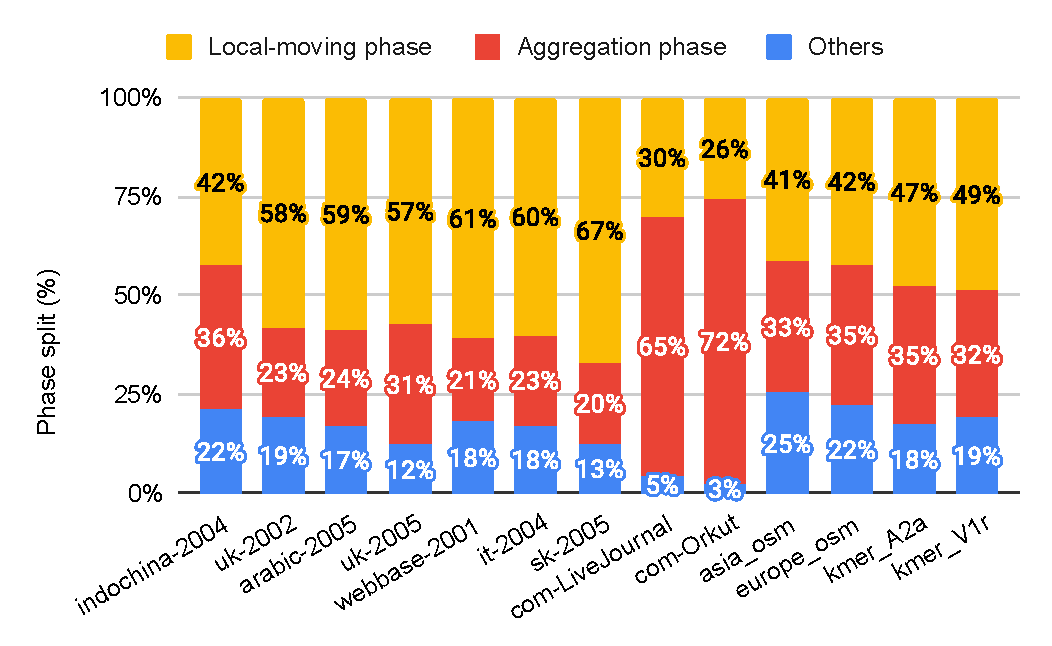
\includegraphics[width=0.48\linewidth]{out/leiden-phases.pdf}
  }
  \subfigure[Pass split]{
    \label{fig:leiden-splits--pass}
    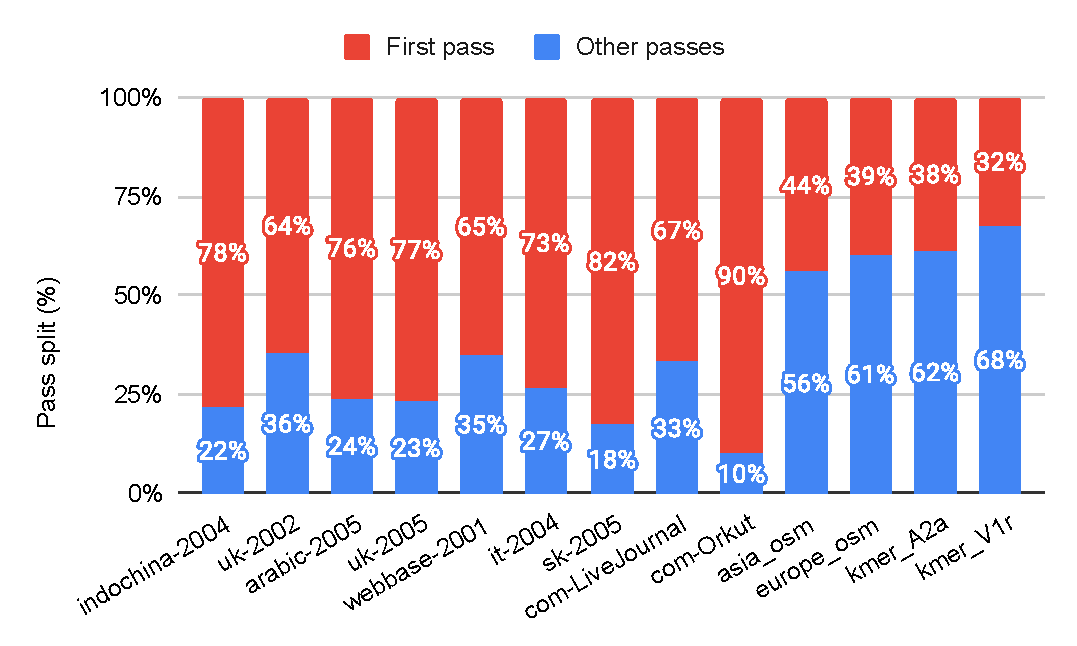
\includegraphics[width=0.48\linewidth]{out/leiden-passes.pdf}
  } \\[-2ex]
  \caption{Phase split of \textit{GVE-Leiden} shown on the left, and pass split shown on the right for each graph in the dataset.}
  \label{fig:leiden-splits}
\end{figure*}

\begin{figure}[hbtp]
  \centering
  \subfigure{
    \label{fig:leiden-hardness--all}
    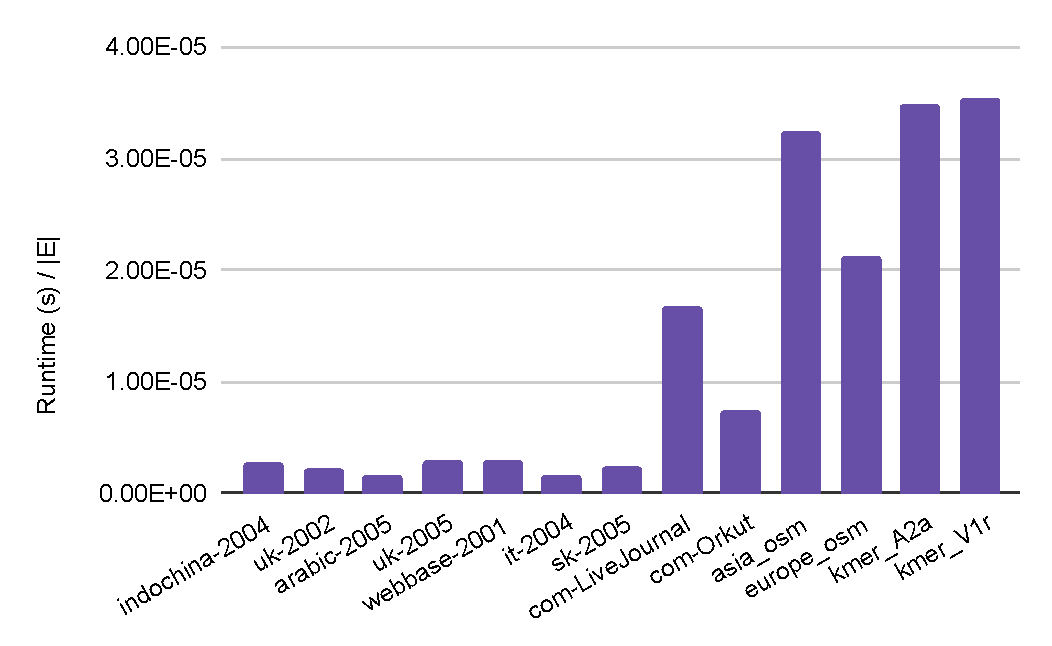
\includegraphics[width=0.98\linewidth]{out/leiden-hardness.pdf}
  } \\[-2ex]
  \caption{Runtime $/ |E|$ factor with \textit{GVE-Leiden} for each graph in the dataset.}
  \label{fig:leiden-hardness}
\end{figure}

\begin{figure}[hbtp]
  \centering
  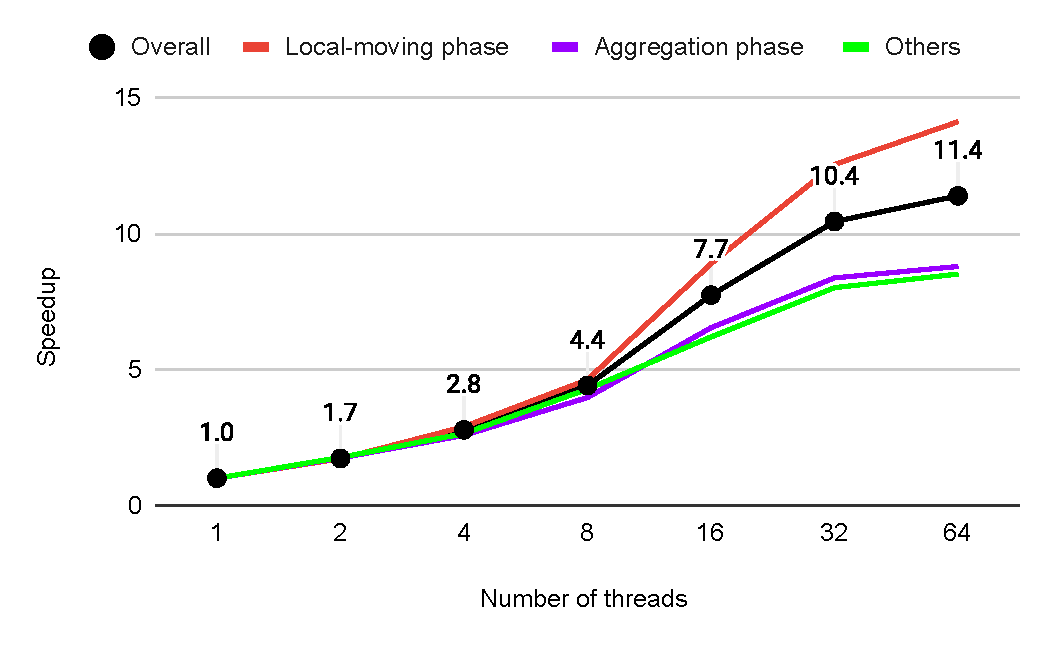
\includegraphics[width=0.98\linewidth]{out/leiden-ss.pdf} \\[-2ex]
  \caption{Overall speedup of \textit{GVE-Leiden}, and its various phases (local-moving, refinement, aggregation, others), with increasing number of threads (in multiples of 2).}
  \label{fig:leiden-ss}
\end{figure}





\subsection{Analyzing Performance of GVE-Leiden}

We now analyze the performance of GVE-Leiden. The phase-wise and pass-wise split of GVE-Leiden is shown in Figures \ref{fig:leiden-splits--phase} and \ref{fig:leiden-splits--pass} respectively. Figure \ref{fig:leiden-splits--phase} reveals that GVE-Leiden devotes a significant portion of its runtime to the local-moving and refinement phases on \textit{web graphs}, \textit{road networks}, and \textit{protein k-mer graphs}, while it dedicates majority of its runtime in the aggregation phase on \textit{social networks}. The pass-wise split, shown in Figure \ref{fig:leiden-splits--pass}, indicates that the first pass is time-intensive for high-degree graphs (\textit{web graphs} and \textit{social networks}), while subsequent passes take precedence in execution time on low-degree graphs (\textit{road networks} and \textit{protein k-mer graphs}).

On average, GVE-Leiden spends $46\%$ of its runtime in the local-moving phase, $19\%$ in the refinement phase, $20\%$ in the aggregation phase, and $15\%$ in other steps (initialization, renumbering communities, dendrogram lookup, and resetting communities). Further, $63\%$ of the runtime is consumed by the first pass of the algorithm, which is computationally demanding due to the size of the original graph (subsequent passes operate on super-vertex graphs). We also observe that graphs with lower average degree (\textit{road networks} and \textit{protein k-mer graphs}) and those with poor community structure (e.g., \verb|com-LiveJournal| and \verb|com-Orkut|) exhibit a higher $\text{runtime}/|E|$ factor, as shown in Figure \ref{fig:leiden-hardness}.




\subsection{Strong Scaling of GVE-Leiden}

Finally, we assess the strong scaling performance of GVE-Leiden. In this analysis, we vary the number of threads from $1$ to $64$ in multiples of $2$ for each input graph, and measure the total time taken for GVE-Leiden to identify communities, encompassing its phase splits (local-moving, refinement, aggregation, and others), repeated five times for averaging. The results are shown in Figure \ref{fig:leiden-ss}. With 32 threads, GVE-Leiden achieves an average speedup of $11.4\times$ compared to a single-threaded execution, indicating a performance increase of $1.6\times$ for every doubling of threads. Nevertheless, scalability is restricted due to the sequential nature of steps/phases in the algorithm. At 64 threads, GVE-Leiden is affected by NUMA effects, resulting in a speedup of only $16.0\times$.
